\section{Position Vectors}

\begin{definition}
  A {\bf position vector} is a vector that represents the position of a point in space relative to the origin, $O$. 
\end{definition}

Let any vector $\vec{v}$ be the position vector of a point $P$ in space. Then, the coordinates of $P$ are given by the components of $\vec{v}$:
\begin{figure}[H]
\centering
   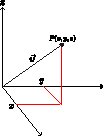
\includegraphics[scale=2.5]{position-vectors.pdf}
   \caption{Position Vector}
   \label{fig:figure-4-position-vector}
\end{figure}

So the position vector of $P$ is given by:
\begin{equation}
  \vec{v} = \begin{bmatrix} x \\ y \\ j \end{bmatrix}  =x\hat{i} + y\hat{j} + k\hat{k}
\end{equation}
\clearpage
